% Options for packages loaded elsewhere
\PassOptionsToPackage{unicode}{hyperref}
\PassOptionsToPackage{hyphens}{url}
%
\documentclass[
  ignorenonframetext,
]{beamer}
\usepackage{pgfpages}
\setbeamertemplate{caption}[numbered]
\setbeamertemplate{caption label separator}{: }
\setbeamercolor{caption name}{fg=normal text.fg}
\beamertemplatenavigationsymbolsempty
% Prevent slide breaks in the middle of a paragraph
\widowpenalties 1 10000
\raggedbottom
\setbeamertemplate{part page}{
  \centering
  \begin{beamercolorbox}[sep=16pt,center]{part title}
    \usebeamerfont{part title}\insertpart\par
  \end{beamercolorbox}
}
\setbeamertemplate{section page}{
  \centering
  \begin{beamercolorbox}[sep=12pt,center]{part title}
    \usebeamerfont{section title}\insertsection\par
  \end{beamercolorbox}
}
\setbeamertemplate{subsection page}{
  \centering
  \begin{beamercolorbox}[sep=8pt,center]{part title}
    \usebeamerfont{subsection title}\insertsubsection\par
  \end{beamercolorbox}
}
\AtBeginPart{
  \frame{\partpage}
}
\AtBeginSection{
  \ifbibliography
  \else
    \frame{\sectionpage}
  \fi
}
\AtBeginSubsection{
  \frame{\subsectionpage}
}

\usepackage{amsmath,amssymb}
\usepackage{lmodern}
\usepackage{iftex}
\ifPDFTeX
  \usepackage[T1]{fontenc}
  \usepackage[utf8]{inputenc}
  \usepackage{textcomp} % provide euro and other symbols
\else % if luatex or xetex
  \usepackage{unicode-math}
  \defaultfontfeatures{Scale=MatchLowercase}
  \defaultfontfeatures[\rmfamily]{Ligatures=TeX,Scale=1}
\fi
% Use upquote if available, for straight quotes in verbatim environments
\IfFileExists{upquote.sty}{\usepackage{upquote}}{}
\IfFileExists{microtype.sty}{% use microtype if available
  \usepackage[]{microtype}
  \UseMicrotypeSet[protrusion]{basicmath} % disable protrusion for tt fonts
}{}
\makeatletter
\@ifundefined{KOMAClassName}{% if non-KOMA class
  \IfFileExists{parskip.sty}{%
    \usepackage{parskip}
  }{% else
    \setlength{\parindent}{0pt}
    \setlength{\parskip}{6pt plus 2pt minus 1pt}}
}{% if KOMA class
  \KOMAoptions{parskip=half}}
\makeatother
\usepackage{xcolor}
\newif\ifbibliography
\setlength{\emergencystretch}{3em} % prevent overfull lines
\setcounter{secnumdepth}{-\maxdimen} % remove section numbering


\providecommand{\tightlist}{%
  \setlength{\itemsep}{0pt}\setlength{\parskip}{0pt}}\usepackage{longtable,booktabs,array}
\usepackage{calc} % for calculating minipage widths
\usepackage{caption}
% Make caption package work with longtable
\makeatletter
\def\fnum@table{\tablename~\thetable}
\makeatother
\usepackage{graphicx}
\makeatletter
\def\maxwidth{\ifdim\Gin@nat@width>\linewidth\linewidth\else\Gin@nat@width\fi}
\def\maxheight{\ifdim\Gin@nat@height>\textheight\textheight\else\Gin@nat@height\fi}
\makeatother
% Scale images if necessary, so that they will not overflow the page
% margins by default, and it is still possible to overwrite the defaults
% using explicit options in \includegraphics[width, height, ...]{}
\setkeys{Gin}{width=\maxwidth,height=\maxheight,keepaspectratio}
% Set default figure placement to htbp
\makeatletter
\def\fps@figure{htbp}
\makeatother

\makeatletter
\makeatother
\makeatletter
\makeatother
\makeatletter
\@ifpackageloaded{caption}{}{\usepackage{caption}}
\AtBeginDocument{%
\ifdefined\contentsname
  \renewcommand*\contentsname{Table of contents}
\else
  \newcommand\contentsname{Table of contents}
\fi
\ifdefined\listfigurename
  \renewcommand*\listfigurename{List of Figures}
\else
  \newcommand\listfigurename{List of Figures}
\fi
\ifdefined\listtablename
  \renewcommand*\listtablename{List of Tables}
\else
  \newcommand\listtablename{List of Tables}
\fi
\ifdefined\figurename
  \renewcommand*\figurename{Figure}
\else
  \newcommand\figurename{Figure}
\fi
\ifdefined\tablename
  \renewcommand*\tablename{Table}
\else
  \newcommand\tablename{Table}
\fi
}
\@ifpackageloaded{float}{}{\usepackage{float}}
\floatstyle{ruled}
\@ifundefined{c@chapter}{\newfloat{codelisting}{h}{lop}}{\newfloat{codelisting}{h}{lop}[chapter]}
\floatname{codelisting}{Listing}
\newcommand*\listoflistings{\listof{codelisting}{List of Listings}}
\makeatother
\makeatletter
\@ifpackageloaded{caption}{}{\usepackage{caption}}
\@ifpackageloaded{subcaption}{}{\usepackage{subcaption}}
\makeatother
\makeatletter
\@ifpackageloaded{tcolorbox}{}{\usepackage[many]{tcolorbox}}
\makeatother
\makeatletter
\@ifundefined{shadecolor}{\definecolor{shadecolor}{rgb}{.97, .97, .97}}
\makeatother
\makeatletter
\makeatother
\ifLuaTeX
  \usepackage{selnolig}  % disable illegal ligatures
\fi
\IfFileExists{bookmark.sty}{\usepackage{bookmark}}{\usepackage{hyperref}}
\IfFileExists{xurl.sty}{\usepackage{xurl}}{} % add URL line breaks if available
\urlstyle{same} % disable monospaced font for URLs
\hypersetup{
  pdftitle={Economía Política},
  hidelinks,
  pdfcreator={LaTeX via pandoc}}

\title{Economía Política}
\subtitle{Unidad 1. Es la política, estúpido! Introducción a la economía
política}
\author{\textbf{Sebastián Freille}\\
sfreille@unc.edu.ar\\
Licenciatura en Economía\\
FCE-UNC}
\date{}

\begin{document}
\frame{\titlepage}
\ifdefined\Shaded\renewenvironment{Shaded}{\begin{tcolorbox}[sharp corners, enhanced, boxrule=0pt, breakable, borderline west={3pt}{0pt}{shadecolor}, frame hidden, interior hidden]}{\end{tcolorbox}}\fi

\begin{frame}
\begin{quote}
Los economistas deben no sólo conocer sus modelos económicos, sino que
también entender de política, intereses, conflictos, pasiones, es decir,
la esencia de la vida colectiva. Por un pequeño período de tiempo, uno
puede realizar cambios a través de decretos: pero para que ellos
persistan, uno debe construir coaliciones y tener gente que los soporte.
Es decir, se debe ser un político.\\
\textbf{{[}Alejandro Foxley, ex Ministro de Finanzas de Chile{]}}
\end{quote}
\end{frame}

\begin{frame}{\textbf{Introducción a la economía política}}
\protect\hypertarget{introducciuxf3n-a-la-economuxeda-poluxedtica}{}
\begin{itemize}
\tightlist
\item
  Economía y política
\item
  Antecedentes, tradiciones y metodología
\item
  Enfoque: limitaciones y considerandos
\end{itemize}

\begin{block}{Economía y política}
\protect\hypertarget{economuxeda-y-poluxedtica}{}
\begin{itemize}
\tightlist
\item
  Economía \(\longrightarrow\) uso óptimo de recursos escasos
\item
  Política \(\longrightarrow\) estudio del poder y la autoridad
\item
  Poder \(\longrightarrow\) habilidad (capacidad) de individuos y/o
  grupos para lograr sus objetivos
\item
  En cualquier estudio que pretenda describir la complejidad de las
  relaciones sociales en sus dimensiones económicas y políticas, estos
  elementos deben analizarse en forma conjunta.
\end{itemize}
\end{block}

\begin{block}{Economía y politica (cont.)}
\protect\hypertarget{economuxeda-y-politica-cont.}{}
\begin{itemize}
\tightlist
\item
  La economía como disciplina nace y se desarrolla como economía
  política (Smith, Ricardo, Marx, JS Mill, Say). La economia neoclásica
  enfoca en \textbf{planificador benevolente} \(\longrightarrow\)
  enfoque normativo
\item
  ¿Cómo y porqué es la política económica como es? ¿Cómo es el proceso
  político de toma de decisiones colectivas por parte de \textbf{agentes
  con preferencias diferentes} \(\longrightarrow\) enfoque positivo
\item
  Esto último es lo que se entiende modernamente por \textbf{economia
  política}
\end{itemize}
\end{block}

\begin{block}{Economía y política: tradiciones}
\protect\hypertarget{economuxeda-y-poluxedtica-tradiciones}{}
\begin{itemize}
\tightlist
\item
  Tres tradiciones nutren a la economia política

  \begin{itemize}
  \tightlist
  \item
    Teoría de la \textbf{política macroeconómica} \(\longrightarrow\)
    exp. racionales, incentivos del \emph{policy maker} y comportamiento
    estratégico. Teórica; instituciones políticas poco realistas
  \item
    Teoría de la \textbf{elección pública} \(\longrightarrow\) finanzas
    públicas, política regulatoria. Eje: problema de agencia entre el
    gobierno (agente) y ciudadanos (principal).
  \item
    Teoría de la \textbf{elección social} \(\longrightarrow\) modelos
    formales de análisis político. Se inicia con los modelos de votación
    espacial y la teoría axiomática de la elección social (Arrow).
    Estudia decisiones colectivas en instituciones políticas
    específicas.
  \end{itemize}
\end{itemize}
\end{block}

\begin{block}{Enfoque metodológico}
\protect\hypertarget{enfoque-metodoluxf3gico}{}
\begin{quote}
Enfoque de la economía política moderna: síntesis Utiliza el enfoque de
equilibrio general de la \textbf{teoría macroeconómica} de la política y
explota las herramientas de la \textbf{teoría de la elección racional}
para el análisis de los problemás principales de la \textbf{teoría de la
elección pública}
\end{quote}
\end{block}

\begin{block}{Enfoque: resumen}
\protect\hypertarget{enfoque-resumen}{}
\begin{itemize}
\tightlist
\item
  Enfoque consiste en aplicar métodos de análisis modernos al ámbito
  político \(\longrightarrow\) politicas económicas resultado de
  interacción entre individuos racionales con preferencias heterogéneas
\item
  Si bien el método en ocasiones suele ser criticado por excesivamente
  formal y racionalista, se pueden incorporar otros paradigmas para
  analizar el efecto de relajar ciertos supuestos.
\end{itemize}
\end{block}

\begin{block}{Las tres I's}
\protect\hypertarget{las-tres-is}{}
\begin{quote}
\textbf{Intereses.} Representados por preferencias de diferentes agentes
por alternativas de políticas. Se modelan al nivel individual.
\end{quote}

\begin{quote}
\textbf{Instituciones.} Restricciones creadas por los humanos que
estructuran la interacción económica, política y social.
\end{quote}

\begin{quote}
\textbf{Ideas.} Incluyen paradigmas, sentimientos públicos, programas y
encuadres que moldean e impactan el tipo y forma de las decisiones
adoptadas.
\end{quote}
\end{block}
\end{frame}

\begin{frame}{\textbf{Heterogeneidad en políticas y outcomes}}
\protect\hypertarget{heterogeneidad-en-poluxedticas-y-outcomes}{}
\begin{itemize}
\tightlist
\item
  Hechos estilizados
\item
  Explicaciones económicas y políticas
\item
  ¿Por qué fracasan los países?
\end{itemize}

\begin{block}{Gasto público y PIB}
\protect\hypertarget{gasto-puxfablico-y-pib}{}
\begin{itemize}
\tightlist
\item
  Existe una relación positiva entre gasto público y PIB per capita con
  alguos \emph{outliers} y posibles no linearidades
\item
  ¿Cómo se explican estas diferencias desde un enfoque puramente
  económico sin considerar la politica?
\item
  Posibles explicaciones \(\longrightarrow\) 1) mayor rol redistributivo
  del Estado; 2) instituciones políticas --presidencialismo vs
  parlamentarismo, mayoritario vs representación proporcional.
\end{itemize}
\end{block}

\begin{block}{Gasto público y PIB (cont.)}
\protect\hypertarget{gasto-puxfablico-y-pib-cont.}{}
\begin{figure}

{\centering 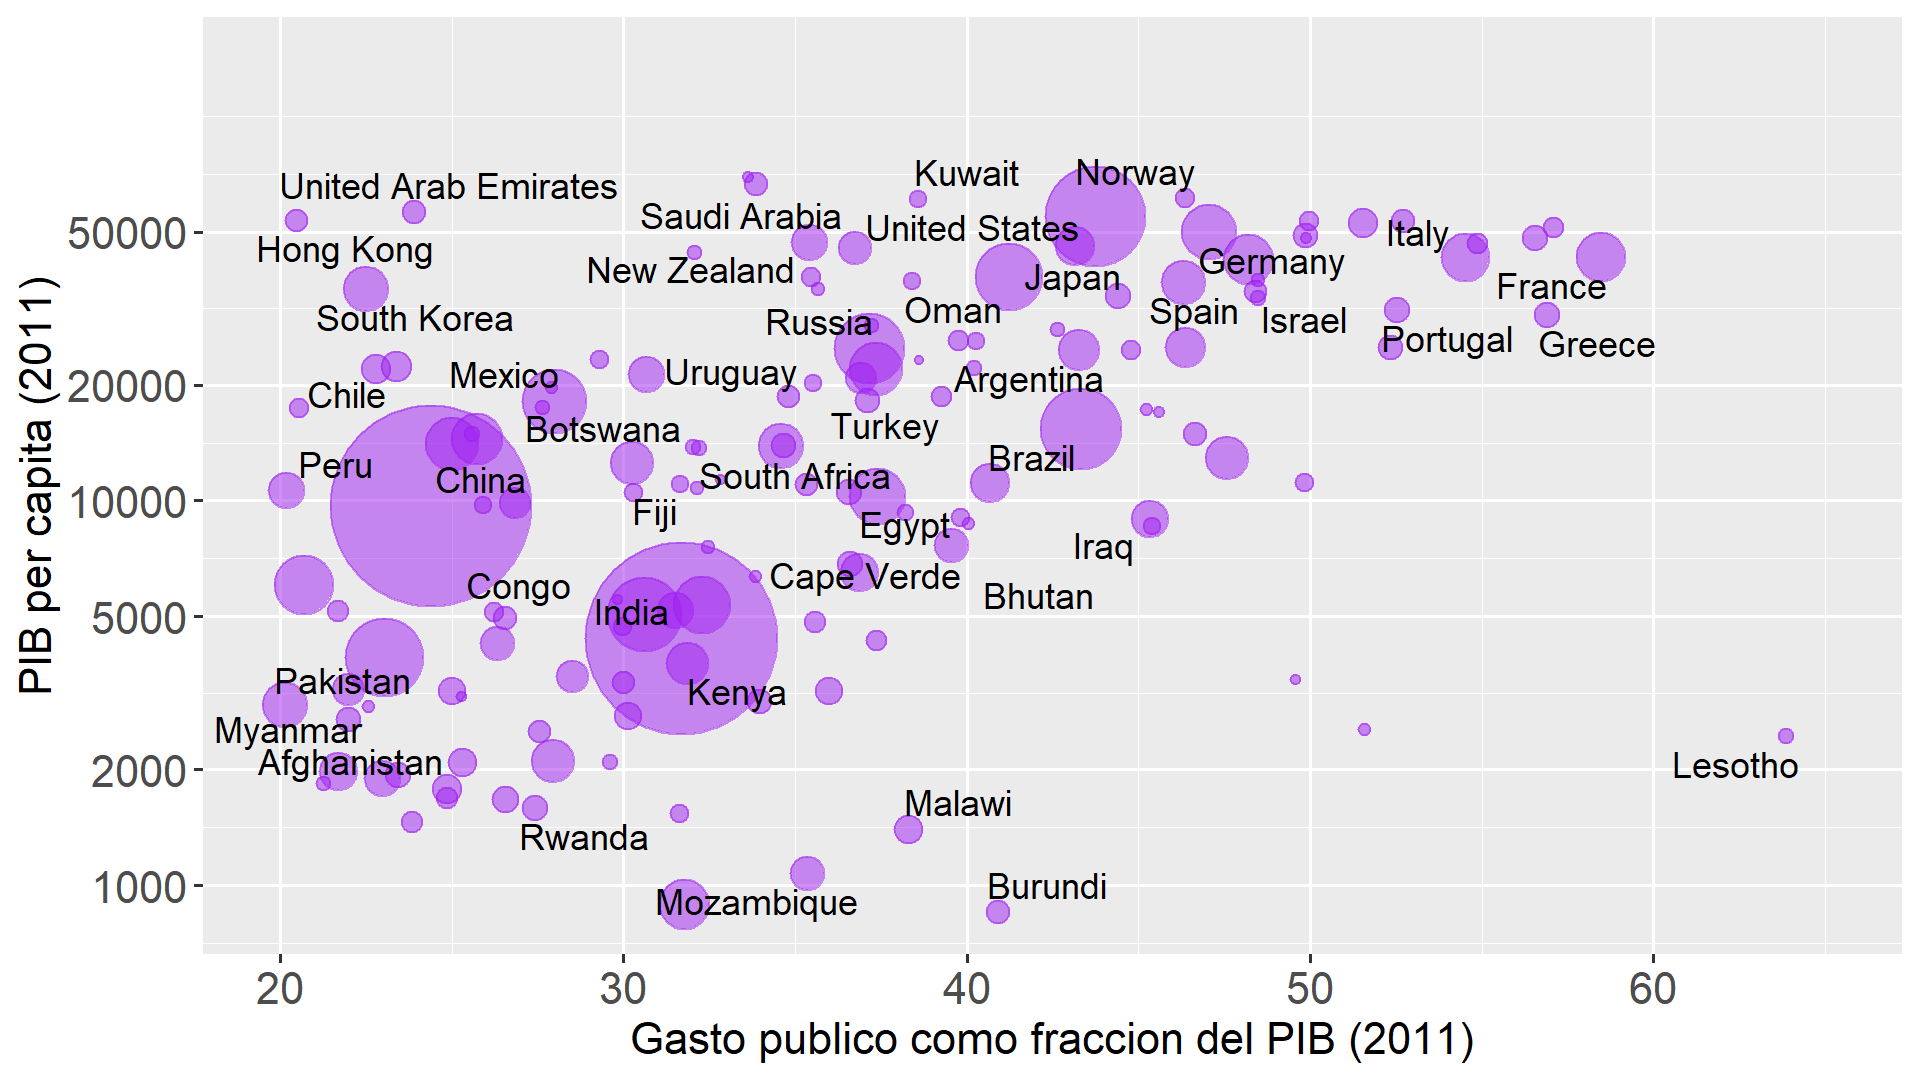
\includegraphics{fig/fig-01-001.png}

}

\caption{Gasto público (\(\%PIB\)) y PBI per capita}

\end{figure}
\end{block}

\begin{block}{Gasto público y PIB: evolución}
\protect\hypertarget{gasto-puxfablico-y-pib-evoluciuxf3n}{}
\begin{itemize}
\tightlist
\item
  Si miramos evolución comparada de largo plazo, observamos claras
  tendencias a mayor participación estatal en la economía
  \(\longrightarrow\) medido tanto por el lado de gastos como de
  recursos y también para diferentes países
\item
  También aquí la política es importante \(\longrightarrow\) expansión y
  fortalecimiento de las democracias en los últimos 150 años
\item
  ¿Diferentes preferencias? ¿Diferentes instituciones?
\end{itemize}
\end{block}

\begin{block}{Gasto público y PIB: evolución (cont.)}
\protect\hypertarget{gasto-puxfablico-y-pib-evoluciuxf3n-cont.}{}
\begin{figure}

{\centering 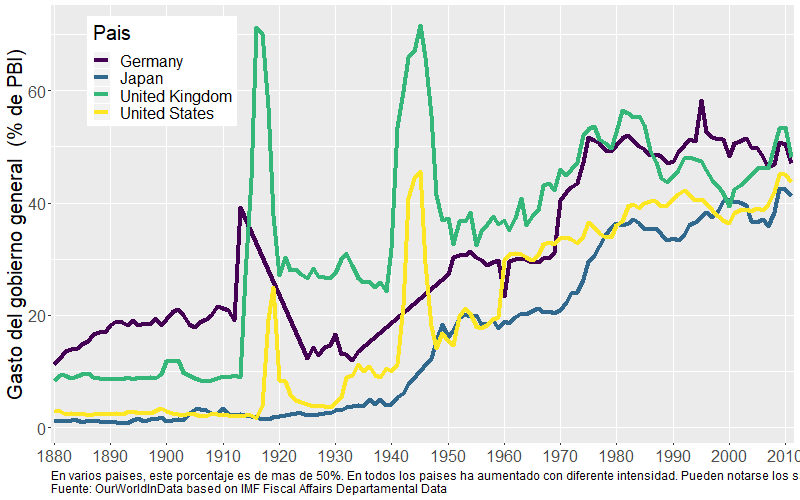
\includegraphics{fig/fig-01-002.png}

}

\caption{Evolución gasto público (\(\%PIB\)) - Paises industriales}

\end{figure}
\end{block}

\begin{block}{Gasto público y PIB: evolución (cont.)}
\protect\hypertarget{gasto-puxfablico-y-pib-evoluciuxf3n-cont.-1}{}
\begin{figure}

{\centering 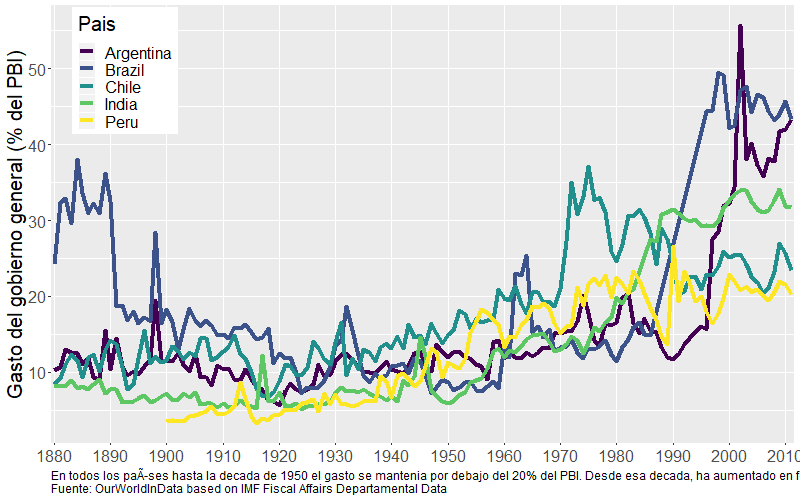
\includegraphics{fig/fig-01-003.png}

}

\caption{Evolución gasto público (\(\%PIB\)) - Países en desarrollo}

\end{figure}
\end{block}

\begin{block}{Tributos y PIB}
\protect\hypertarget{tributos-y-pib}{}
\begin{itemize}
\tightlist
\item
  Países pobres versus ricos con similar recaudación tributaria --ie.
  tamaño del Estado- \(\longrightarrow\) Lesotho/Alemania
\item
  Países con similar riqueza pero diferente rol del Estado
  \(\longrightarrow\) Oman y Arabia Saudita / EEUU / Noruega
\item
  Economia puede explicar algunas diferencias \(\longrightarrow\) ley de
  Wagner, efecto ``umbral''
\item
  Varias teorías explicativas desde el estudio de la política
  \(\longrightarrow\) 1) maldición de los recursos, 2) corrupción, 3)
  incentivos político-electorales
\end{itemize}
\end{block}

\begin{block}{Tributos y PIB (cont.)}
\protect\hypertarget{tributos-y-pib-cont.}{}
\begin{figure}

{\centering 
\includegraphics{fig/fig-01-004.png}

}

\caption{Recaudacion tributaria (\(\%PIB\)) y PBI per capita}

\end{figure}
\end{block}

\begin{block}{Tributos y PIB (cont.)}
\protect\hypertarget{tributos-y-pib-cont.-1}{}
\begin{figure}

{\centering 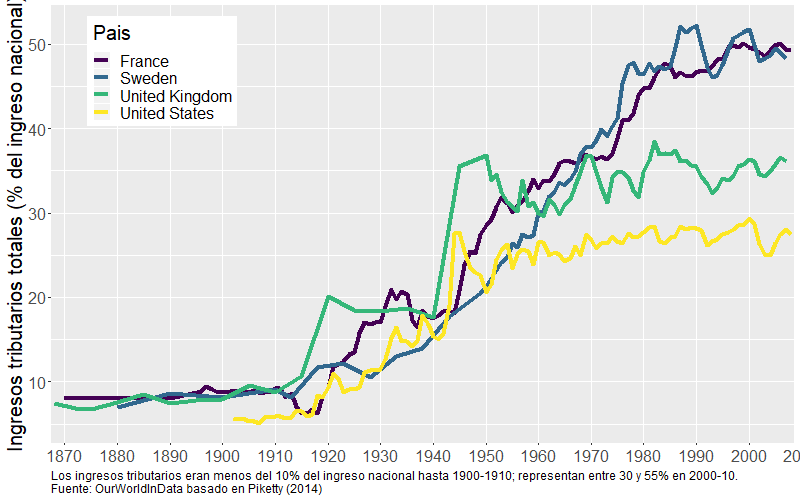
\includegraphics{fig/fig-01-005.png}

}

\caption{Evolución recaudación tributaria (\(\%PIB\)) - Países
industriales}

\end{figure}
\end{block}
\end{frame}

\begin{frame}{\textbf{``It's politics''}}
\protect\hypertarget{its-politics}{}
\begin{itemize}
\tightlist
\item
  Individuos heterogeneos en varios aspectos
\item
  Desvíos de los teoremas de bienestar
\item
  Tipos de heterogeneidad e implicancias
\item
  ¿Cómo se deciden los ``pesos''?
\end{itemize}

\begin{block}{Heterogeneidad de intereses}
\protect\hypertarget{heterogeneidad-de-intereses}{}
\begin{itemize}
\tightlist
\item
  Un aspecto relevante de la política es en lo que hace a la
  \textbf{heterogeneidad de intereses}
\item
  Restricciones políticas derivadas de ello implica que las políticas
  adoptadas en la práctica \textbf{no son óptimas}
\item
  Implicaciones positivas \(\longrightarrow\) si la política óptima se
  encuentra no resulta cierto que esta se implementa (implícito en la
  \emph{economía del bienestar})
\item
  Implicaciones normativas \(\longrightarrow\) ¿cómo pueden diseñarse
  instituciones y políticas para lograr ciertos objetivos?
\end{itemize}
\end{block}

\begin{block}{Los teoremas del bienestar}
\protect\hypertarget{los-teoremas-del-bienestar}{}
\begin{quote}
\textbf{Primer teorema del bienestar (1TDB)} \(\longrightarrow\)
cualquier asignación que resulta de un equilibrio competitivo es
Pareto-eficiente
\end{quote}

\begin{quote}
\textbf{Segundo teorema del bienestar (2TDB)} \(\longrightarrow\) bajo
preferencias convexas, cualquier asignación Pareto-eficiente
\emph{puede} resultar en un equilibrio competitivo (mediante una
reasignación de las dotaciones iniciales)
\end{quote}

\begin{itemize}
\tightlist
\item
  Los teoremas son las dos espadas principales de la economía del
  bienestar en cuanto orientaciones de política económica --en este
  sentido la economía del bienestar es un asunto de \emph{economía
  normativa} {[}Blaug (1978), Price (1977){]}
\end{itemize}
\end{block}

\begin{block}{1TDB: Eficiencia asignativa}
\protect\hypertarget{tdb-eficiencia-asignativa}{}
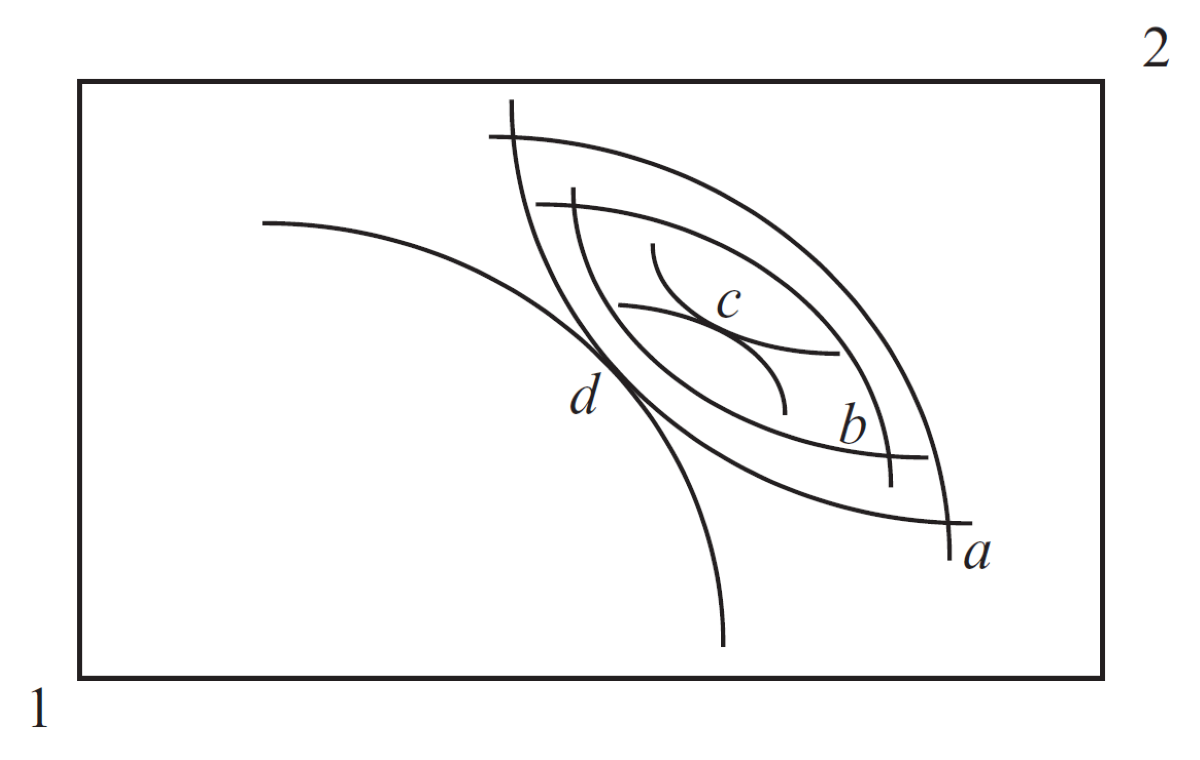
\includegraphics[width=0.45\textwidth,height=\textheight]{fig/fig-01-006.png}

\includegraphics[width=0.45\textwidth,height=\textheight]{fig/fig-01-007.png}
\end{block}

\begin{block}{2TDB: Eficiencia en (re)distribución}
\protect\hypertarget{tdb-eficiencia-en-redistribuciuxf3n}{}
\begin{figure}

{\centering 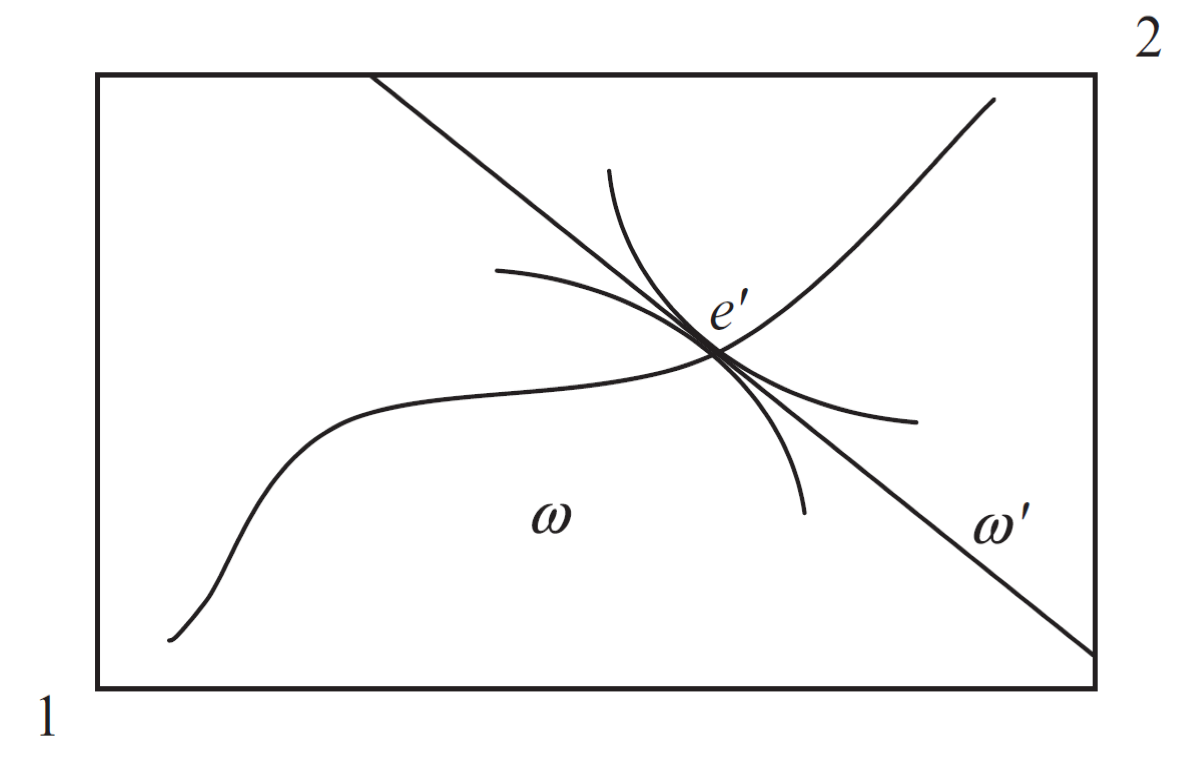
\includegraphics{fig/fig-01-008.png}

}

\caption{Cada dotación origina un equilibrio}

\end{figure}
\end{block}

\begin{block}{``Todos los modelos están mal\ldots{}''}
\protect\hypertarget{todos-los-modelos-estuxe1n-mal}{}
\begin{itemize}
\tightlist
\item
  Eficiencia Paretiana \(\longrightarrow\) deseable pero débil e
  insuficiente --una persona consumo todo y el resto nada será
  Pareto-eficiente
\item
  Condiciones muy estrictas --externalidades, competencia, información
  perfecta e individuos racionales
\item
  El 2TDB asume que no hay \textbf{\emph{trade-off} eficiencia versus
  equidad}.
\item
  Es un resultado con profundas implicancias sobre cómo pensar la
  organización de la actividad económica en cualquier economía
  {[}Stiglitz (1991){]}
\end{itemize}
\end{block}

\begin{block}{Sobre la redistribución inicial}
\protect\hypertarget{sobre-la-redistribuciuxf3n-inicial}{}
\begin{itemize}
\tightlist
\item
  El 2TDB supone \emph{implícitamente} que la redistribución inicial de
  la dotación/riqueza se hace via \textbf{transferencias
  \emph{lump-sum}} --no voluntarias- entre consumidores {[}en la
  práctica esto sería un \textbf{impuesto \emph{lump-sum}}{]}
\item
  El tamaño de la transferencia no se ve afectado por cambio en la
  conducta --no hay efecto sustitución, sólo efecto ingreso.
\item
  El problema es que este mecanismo es inviable --las dotaciones
  iniciales no pueden ser observadas por el gobierno
\end{itemize}
\end{block}

\begin{block}{Sobre la redistribución inicial (cont.)}
\protect\hypertarget{sobre-la-redistribuciuxf3n-inicial-cont.}{}
\begin{itemize}
\tightlist
\item
  Cada consumidor tiene dotación y preferencias. La dotación de
  consumidor \(h\) es \(w^{h}=(w_{1}^{h},w_{2}^{h})\) donde
  \(w_{i}^{h} \geq 0\) el stock inicial de \(i\) de \(h\).
\item
  Dados los precios \(p_{1}\) y \(p_{2}\), un plan de consumo para \(h\)
  es \(x^{h}=(x_{1}^{h},x_{2}^{h})\) y satisface la RP.
  \[\begin{aligned}
  p_{1}x_{1}^{h}+p_{2}x_{2}^{h}=p_{1}w_{1}^{h}+p_{2}w_{2}^{h}
  \end{aligned}\]
\item
  La función de utilidad del consumidor \(h\) es: \[\begin{aligned}
  U^{h}=U^{h}(x_{1}^{h},x_{2},^{h})
  \end{aligned}\]
\end{itemize}
\end{block}

\begin{block}{Sobre la redistribución inicial (cont.)}
\protect\hypertarget{sobre-la-redistribuciuxf3n-inicial-cont.-1}{}
\begin{figure}

{\centering 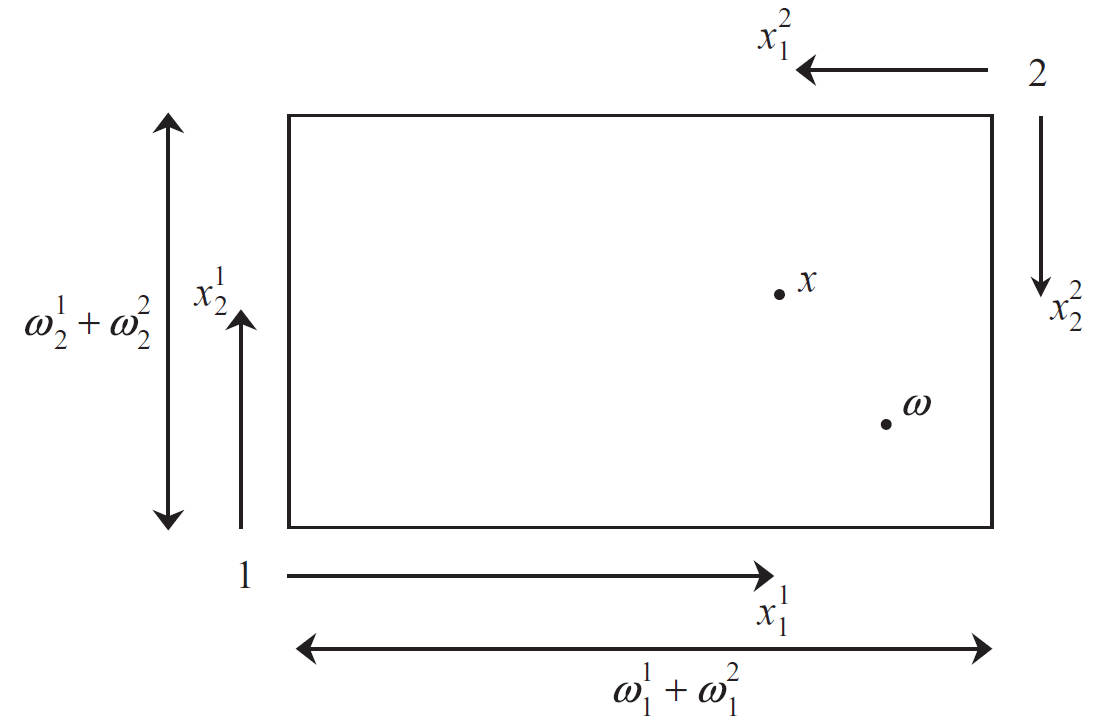
\includegraphics{fig/fig-01-010.png}

}

\caption{Dotaciones y consumos}

\end{figure}
\end{block}

\begin{block}{Sobre la redistribución inicial (cont.)}
\protect\hypertarget{sobre-la-redistribuciuxf3n-inicial-cont.-2}{}
\begin{itemize}
\tightlist
\item
  En el punto inicial, el ingreso de \(h\) es \(\hat{p}w^{h}\). El valor
  de la transferencia requerida para \(h\) es igual a: \[\begin{aligned}
  M^{h}-\hat{p}w^{h}=\hat{p}x^{h}-\hat{p}w^{h}
  \end{aligned}\]
\item
  Una forma de hacerlo sería transferir \(\tilde{x}_{1}^{1}\) del bien 1
  del consumidor 1 al 2 --\(\tilde{x}_{h}^{i}\) denota el consumo
  \emph{neto} del bien \(i\), es decir \(x_{h}^{1}-w_{h}^{1}\).\\
\item
  Problema \(\longrightarrow\) es imposible transferir dotaciones --la
  dotacion de cada persona es su oferta de trabajo --por esa razón, se
  modelan como \textbf{impuestos de suma fija}.
\end{itemize}
\end{block}

\begin{block}{Sobre la redistribución inicial (cont.)}
\protect\hypertarget{sobre-la-redistribuciuxf3n-inicial-cont.-3}{}
\begin{figure}

{\centering 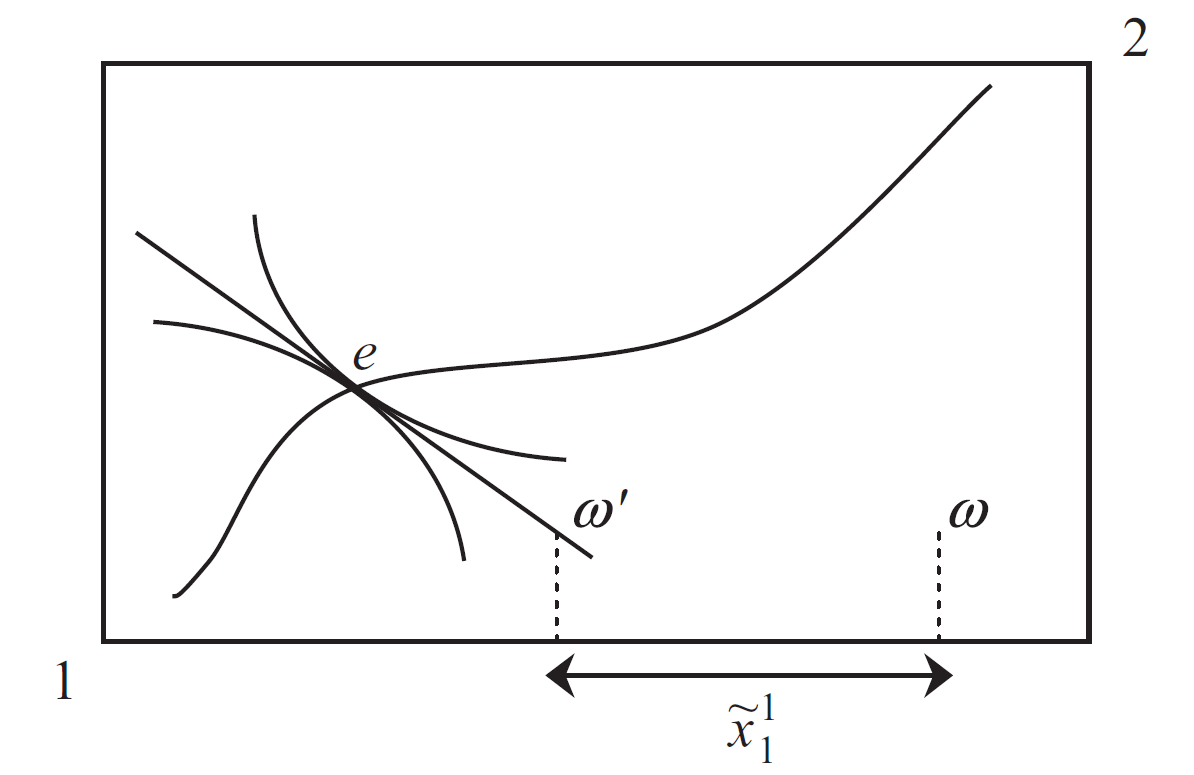
\includegraphics{fig/fig-01-009.png}

}

\caption{Implica redistribución de dotación}

\end{figure}
\end{block}

\begin{block}{Sobre la redistribución inicial (cont.)}
\protect\hypertarget{sobre-la-redistribuciuxf3n-inicial-cont.-4}{}
\begin{itemize}
\tightlist
\item
  Suponga que ambos consumidores venden su dotación (trabajo) al precio
  \(\hat{p}\) \(\longrightarrow\) ingresos de \(\hat{p}w^{1}\) y
  \(\hat{p}w^{2}\)
\item
  Ahora, con impuestos, el consumidor 1 pagaría \[\begin{aligned}
  T^{1}=\hat{p}\tilde{x}_{1}^{1}
  \end{aligned}\]
\item
  y le daria ese monto al consumidor 2, por lo que este pagaría un
  impuesto negativo (subsidio) igual a
  \(T^2=-\hat{p}\tilde{x}_{1}^{1}=-T^{1}\)
\item
  El par de impuestos \(\left(T^{1},T^{2}\right)\) mueve la RP igual que
  las transferencias --el \textbf{impuesto de suma fija no reduce la
  suma de dotaciones iniciales}; redistribución sin costo de eficiencia
  \(\longrightarrow\) impuestos perfectos!
\end{itemize}
\end{block}

\begin{block}{Falacia del 2TDB}
\protect\hypertarget{falacia-del-2tdb}{}
\begin{quote}
Se puede alcanzar cualquier resultado eficiente en el sentido de Pareto
a través de (1) redistribución de las dotaciones iniciales (impuestos
\emph{lump-sum}) y luego (2) dejar que los mercados actúen libremente
\end{quote}

\begin{itemize}
\tightlist
\item
  Pero la redistribucion de dotaciones iniciales no es viable (problema
  de información) \(\longrightarrow\) el gobierno debe usar impuestos y
  transferencias distorsivas.
\item
  Esto implica de facto la \textbf{existencia de un trade-off eficiencia
  y equidad}
\end{itemize}
\end{block}

\begin{block}{Falacia del 2TDB (cont.)}
\protect\hypertarget{falacia-del-2tdb-cont.}{}
\begin{quote}
Suponga que la economía hay un 50\% de gente incapacitada para trabajar
(ingresos \(0\)) y 50\% de personas que pueden trabajar y ganar \(100\)
\end{quote}

\begin{itemize}
\tightlist
\item
  \textbf{Resultado mercado.} Incapacitados ganan \(0\), resto gana
  \(100\)
\item
  \textbf{Resultado 2do TdB.} El gobierno puede distinguir incapacitados
  de capacitados. Pone un impuesto de \(50\) a los capacitados y le da
  \(50\) a cada incapacitado --los capacitados continuan trabajando.
\item
  \textbf{Resultado real.} El gobierno no puede distinguir entre grupos.
  El combo de un impuesto de \(50\) sobre trabajadores y de un subsidio
  de \(50\) sobre no trabajadores destruye todos los incentivos a
  trabajar. El gobiern no puede hacer redistribución completa
  --trade-off entre equidad y eficiencia.
\end{itemize}
\end{block}
\end{frame}

\begin{frame}{\textbf{Aplicación: Equilibrio con y sin política}}
\protect\hypertarget{aplicaciuxf3n-equilibrio-con-y-sin-poluxedtica}{}
\begin{itemize}
\tightlist
\item
  No hay política: problema técnico
\item
  Con política: modelar la heterogeneidad
\item
  Heterogeneidad \emph{ex-ante}
\item
  Heterogeneidad \emph{ex-post}
\item
  El problema de economía política
\end{itemize}

\begin{block}{Equilibrio sin política}
\protect\hypertarget{equilibrio-sin-poluxedtica}{}
\begin{itemize}
\tightlist
\item
  Basado en Drazen (2000) y Ferguson/Querubin (2018)
\item
  Suponga un \textbf{individuo representativo}, Ana quien debe elegir
  cuánto destinar de sus recursos iniciales \(A_{o}\) para sus
  vacaciones de este año y el próximo
\item
  Note que no hay problema político (no conflicto de intereses) sino uno
  técnico
\item
  ¿Cuál es la manera óptima de dividir los recursos entre de vacaciones
  (presente y futuro)?
\end{itemize}
\end{block}

\begin{block}{Equilibrio sin política (cont.)}
\protect\hypertarget{equilibrio-sin-poluxedtica-cont.}{}
\begin{itemize}
\tightlist
\item
  Sea \(u(x_{t})\) la utilidad de Ana por destinar \(x\) a sus
  vacaciones en \(t\) con \(u'>0\) y \(u''<0\). El parámetro \(\beta\)
  compara utilidades en distintos momentos --una unidad de utilidad hoy
  es igual a \(\beta\) unidades de utilidad mañana {[}\(0<\beta<1\){]}
\item
  Problema: \[\max_{x_{t},x_{t+1},s} u(x_{t})+\beta u(x_{t+1})\]
\item
  sujeto a: \[\begin{aligned}
        A_{0}(1-s)&=x_{t} \\
       sA_{0}(1+r_{t})&=x_{t+1} 
        \end{aligned}\]
\end{itemize}
\end{block}

\begin{block}{Equilibrio sin política (cont.)}
\protect\hypertarget{equilibrio-sin-poluxedtica-cont.-1}{}
\begin{itemize}
\tightlist
\item
  Sustituyendo las restricciones:
  \[\max_{x_{t}}u(x_{t})+\beta((A_{o}-x_{t})(1+r_{t}))\]
\item
  Y la solución de esto es: \[u'(x_{t})=\beta(1+r_{t})u'(x_{t+1})\]
\item
  ¿Interpretación de esta solución (ecuación de Euler)?
\end{itemize}
\end{block}

\begin{block}{Equilibrio con política: \emph{ex-ante}}
\protect\hypertarget{equilibrio-con-poluxedtica-ex-ante}{}
\begin{itemize}
\tightlist
\item
  \textbf{Con individuos heterogéneos ex-ante} \(\longrightarrow\)
  preferencias diferentes por consumo presente/futuro {[}dos tipos de
  heterogeneidad: \emph{ex ante} y \emph{ex post}{]}
\item
  Los recursos son los mismos que antes pero ahora hay dos individuos,
  Ana (A) y Juan (J) y sea \(\beta^{A}>\beta^{J}\) {[}Juan es más
  impaciente que Ana{]}
\item
  Problema \(\longrightarrow\) maximizar la función de bienestar social
  (suma ponderada de utilidades individuales) \(\longrightarrow\)
  \(\alpha\) ponderación de cada individuo
\end{itemize}
\end{block}

\begin{block}{Equilibrio con política: \emph{ex-ante} (cont.)}
\protect\hypertarget{equilibrio-con-poluxedtica-ex-ante-cont.}{}
\begin{itemize}
\tightlist
\item
  Problema (neoclasico):
  \[\max_{x_{t},x_{t+1},s} \alpha\left[u(x_{t})+\beta^{A}u(x_{t+1})\right] + (1-\alpha)\left[u(x_{t})+\beta^{J}u(x_{t+1})\right]\]
\item
  sujeto a: \[A_{0}=x_{t}+\frac{x_{t+1}}{(1+r_{t})}\]
\item
  si el bien ``vacaciones'' es no rival --unica fuente de conflicto la
  diferencia ex-ante en el grado de impaciencia de cada uno
\end{itemize}
\end{block}

\begin{block}{Equilibrio con política: \emph{ex-ante} (cont.)}
\protect\hypertarget{equilibrio-con-poluxedtica-ex-ante-cont.-1}{}
\begin{itemize}
\tightlist
\item
  Sustituyendo las restricciones:
  \[u'(x_{t})=(1+r_{t})[\alpha \beta^{A}+(1-\alpha)\beta^{J}]u'(x_{t+1})\]
\item
  Para diferentes \(\alpha\) trazamos \textbf{curva de contrato} con
  asignaciones de \(x_{t}\) y \(x_{t+1}\) eficientes en sentido de
  Pareto
\item
  Varios problemas con esto: 1) cada persona requiere un \(\alpha\) mas
  alto, 2) ¿cómo se determina \(\alpha\), 3) ¿cómo afecta el valor de
  \(\alpha\) a la asignación de recursos, 4) ¿estaremos sobre la curva
  de contrato?
\end{itemize}
\end{block}

\begin{block}{Equilibrio con política: \emph{ex-post}}
\protect\hypertarget{equilibrio-con-poluxedtica-ex-post}{}
\begin{itemize}
\tightlist
\item
  \textbf{Sin individuos heterogéneos ex-ante} \(\longrightarrow\)
  problema converge al del individuo representativo PERO las vacaciones
  no son un bien no rival. El problema es: \[\begin{aligned}
    \max_{x_{t},x_{t+1},s} & \alpha\left[u(\lambda x_{t})+\beta u(\lambda
          x_{t+1})\right] \\ & +(1-\alpha)\left[u((1-\lambda) x_{t})+\beta u((1-\lambda) x_{t+1})\right]
          \end{aligned}\]
\item
  sujeto a {[}\(\lambda\) porcentaje que disfruta Juan del gasto
  \(x\){]} \[\begin{aligned}
                    A_{0}(1-s)&=x_{t}=\lambda x_{t}+(1-\lambda)x_{t} \\
            sA_{0}(1+r_{t})&=x_{t+1}=\lambda x_{t+1}+(1-\lambda)x_{t+1} 
          \end{aligned}\]
\end{itemize}
\end{block}

\begin{block}{Equilibrio con política: \emph{ex-post} (cont.)}
\protect\hypertarget{equilibrio-con-poluxedtica-ex-post-cont.}{}
\begin{itemize}
\tightlist
\item
  Resolviendo: \[\begin{aligned}
    \alpha \lambda u'(\lambda
          x_{t})+(1-\alpha)(1-\lambda)u'((1-\lambda)x_{t})= \\
          \beta(1+r_{t})\left[\alpha \lambda u'(\lambda
          x_{t+1})+(1-\alpha)(1-\lambda)u'((1-\lambda)x_{t+1})\right]
        \end{aligned}\]
\item
  Note que \(\alpha\) es crucial \(\longrightarrow\) pero ahora
  \(\lambda\) también lo es {[}aún suponiendo que \(\alpha=0.5\) existe
  conflicto de interés{]} \[\begin{aligned}
  \lambda u'(\lambda
              x_{t})+(1-\lambda)u'((1-\lambda)x_{t})= \\
              \beta(1+r_{t})\left[\lambda u'(\lambda
          x_{t+1})+(1-\lambda)u'((1-\lambda)x_{t+1})\right]
              \end{aligned}\]
\item
  Si \(\lambda=1\), el resultado seria preferido por Juan y si
  \(\lambda=0\) el resultado sería preferido por Ana.
\end{itemize}
\end{block}

\begin{block}{Equilibrio con política: \emph{ex-post} (cont.)}
\protect\hypertarget{equilibrio-con-poluxedtica-ex-post-cont.-1}{}
\begin{itemize}
\tightlist
\item
  Cuando no hay heterogeneidad, el problema es trivial
  \(\longrightarrow\) problema técnico depende de parámetros subjetivos
\item
  Cuando hay heterogeneidad en preferencias (\emph{ex ante})
  \(\longrightarrow\) como se ponderan utilidades individuales
  {[}\(\alpha\) exógeno{]}
\item
  Cuando hay heterogeneidad en distribución (\emph{ex post})
  \(\longrightarrow\) como se ponderan utilidades invididuales y como se
  distribuye/asigna las cantidades consumidas del bien
\item
  ¿Cómo se determinan los parámetros \(\alpha\) y \(\lambda\) en la
  práctica? No a través del mercado sino del proceso político
\end{itemize}
\end{block}

\begin{block}{Economía y política: todo junto}
\protect\hypertarget{economuxeda-y-poluxedtica-todo-junto}{}
\begin{itemize}
\tightlist
\item
  Una persona, un voto \(\longrightarrow\) \textbf{democracia}
\item
  Un dólar, un voto \(\longrightarrow\) \textbf{mercado}
\item
  Función objetivo del gobierno incluye ambos \[\begin{aligned}
            G&=f(W,C)=\alpha W+\sum_{i}C_{i}
            \end{aligned}\]
\item
  \(W\) es bienestar agregado; \(C_{i}\) es dinero aportado por grupo
  \(i\) --\(\alpha\) ponderador del bienestar agregado.
\end{itemize}
\end{block}

\begin{block}{Economía y política: todo junto (cont.)}
\protect\hypertarget{economuxeda-y-poluxedtica-todo-junto-cont.}{}
\begin{figure}

{\centering 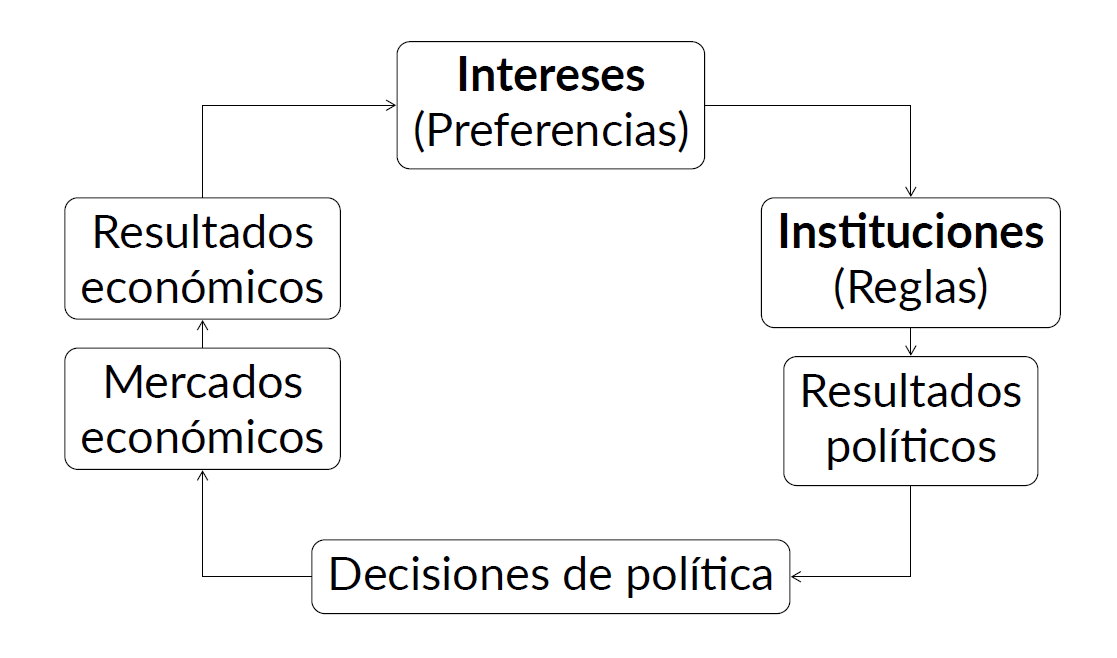
\includegraphics{fig/fig-01-011.png}

}

\caption{Economía política de la política económica}

\end{figure}
\end{block}

\begin{block}{Recap}
\protect\hypertarget{recap}{}
\begin{itemize}
\tightlist
\item
  La política económica en las sociedades modernas no puede explicarse
  sólamente en base a teorías y evidencias económicas
  \(\longrightarrow\) introducir la política explícitamente en el
  análisis
\item
  Hay varias formas de introducir la política \(\longrightarrow\)
  optamos por la aproximación de la nueva economia política
\item
  Pondremos el énfasis en algunos sencillos modelos teóricos --de
  comportamiento-- pero ilustraremos el análisis con evidencias
  empíricas
\end{itemize}
\end{block}
\end{frame}



\end{document}
